\chapter{Slope and Rates of Changes}

\section{The Slope of a Line}

\begin{enumerate}
    \item measure the "steepness" of a line
    \item how quickly a line rises (or falls) as we move from left to right
    \item if a line lies in a coordinate plane, then the run is change in the x-coordinate and the rise is the corresponding change in the y-coordinate between any two points on the line.
\end{enumerate}

\begin{theorem}
The slope m of a non-vertical line that passes through the point $A(x_1, y_1)$ and $B(x_2, x_2)$ is 

\begin{equation}
\label{eq:1}
slope = \frac{rise}{run}=\frac{y_2 - y_1}{x_2 - x_1}
\end{equation}

\begin{flushleft}
The slope of a vertical line is not define.
\end{flushleft}

\end{theorem}

\begin{figure}[h]
    \centering
    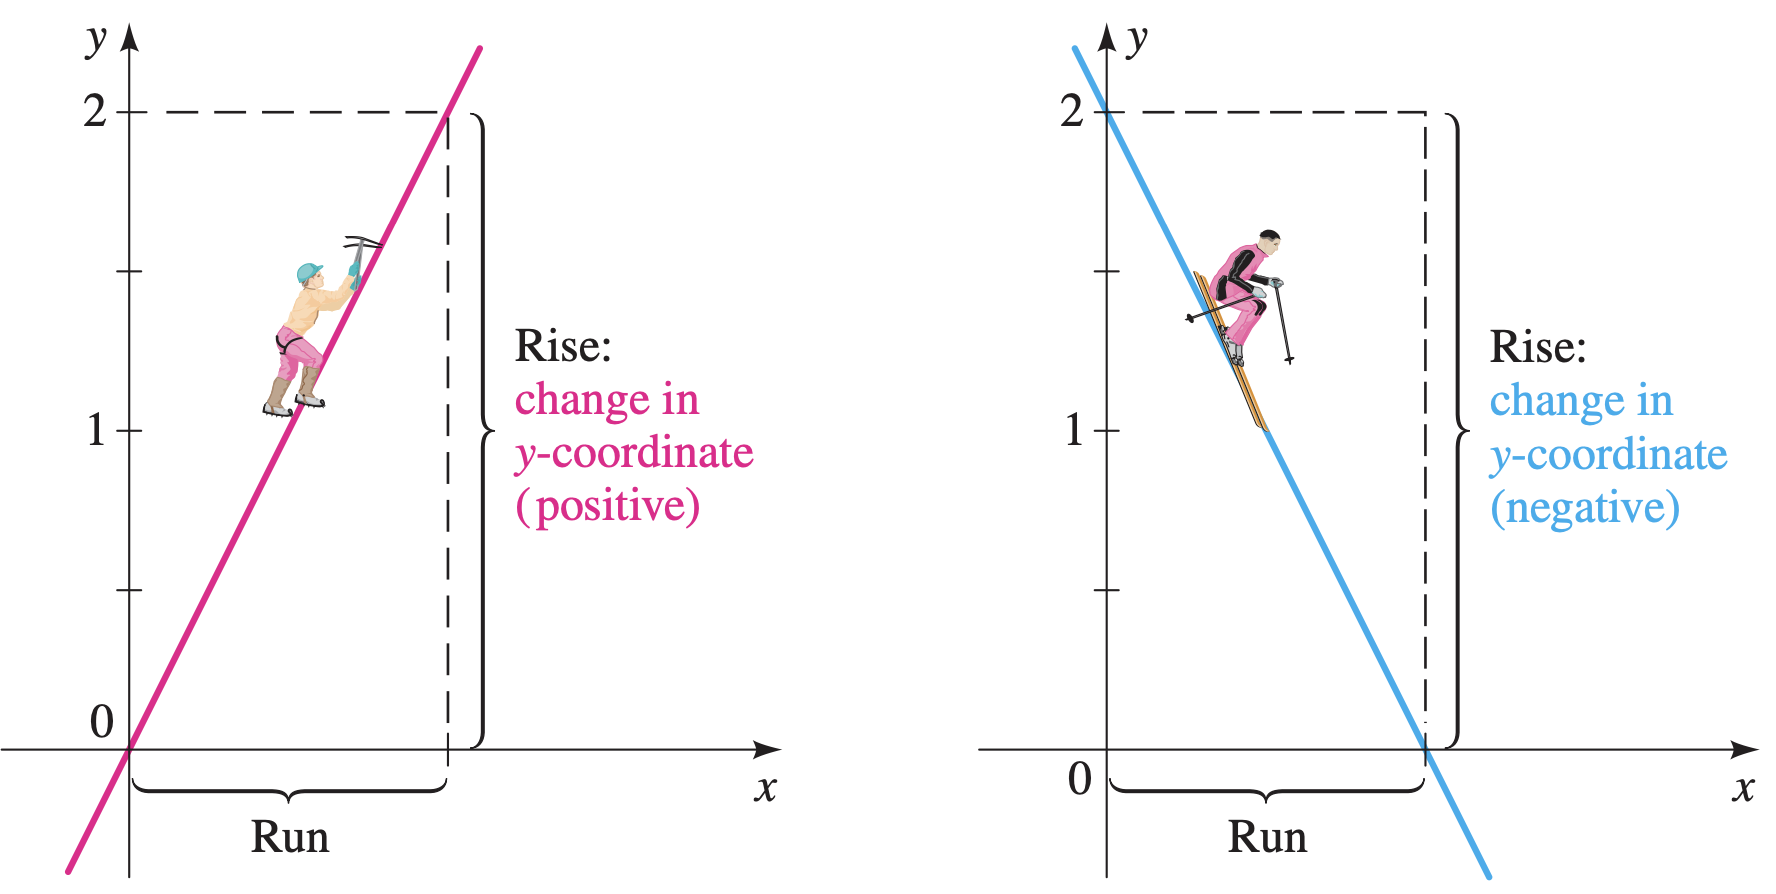
\includegraphics[scale=0.3]{chapter001/figures/fig001}
    \caption{Rise and Run}
    \label{fig:Fig1}
\end{figure}

\newtcolorbox{mybox}[1]{colback=blue!5!white,colframe=blue!75!black,fonttitle=\bfseries,title=#1}
\begin{mybox}{Warning}
The slope is independent of which two points are chosen on the line.
\end{mybox}

\begin{figure}[h]
    \centering
    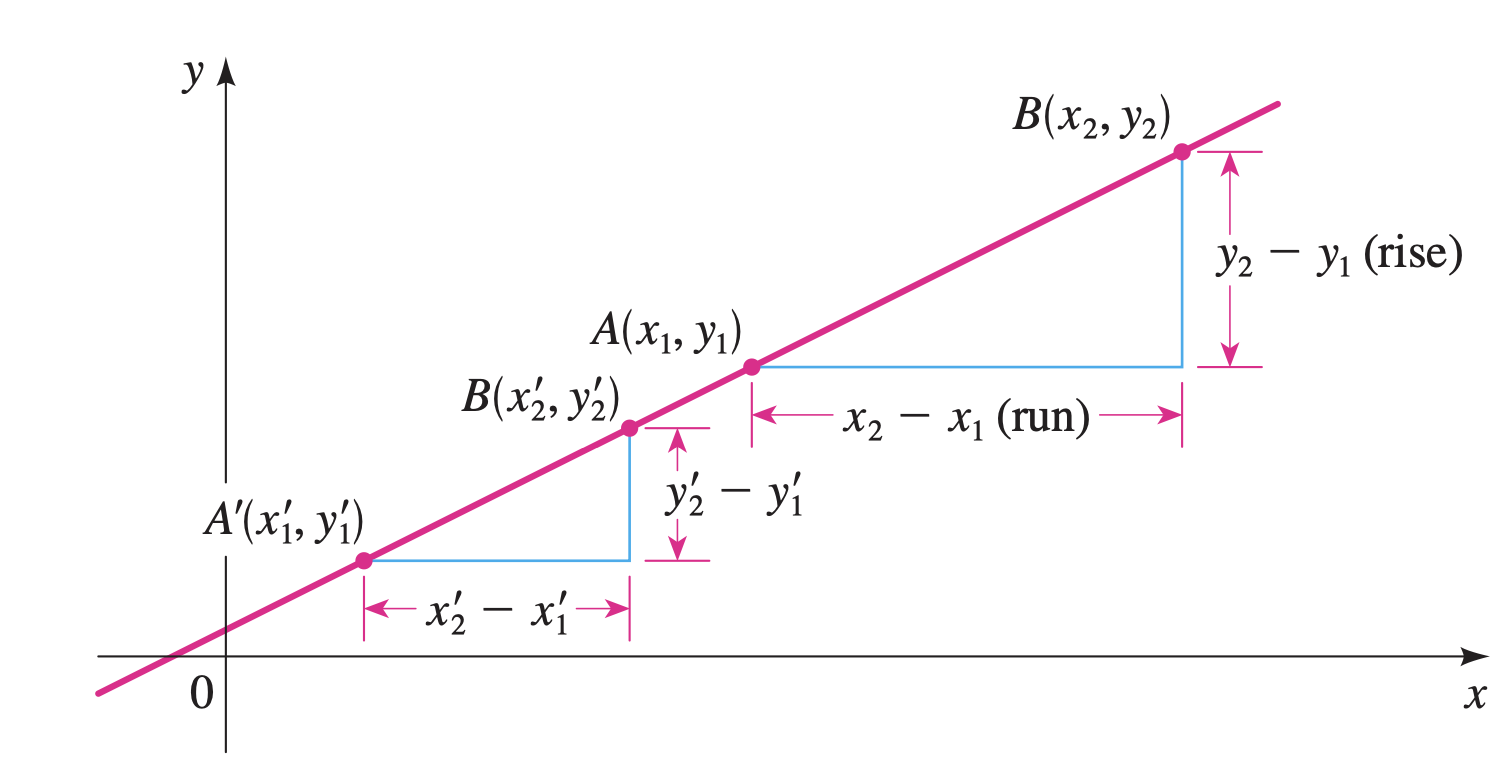
\includegraphics[scale=0.3]{chapter001/figures/fig002}
    \caption{The slope of a vertical line is not define}
    \label{fig:Fig2}
\end{figure}

\begin{figure}[h]
    \centering
    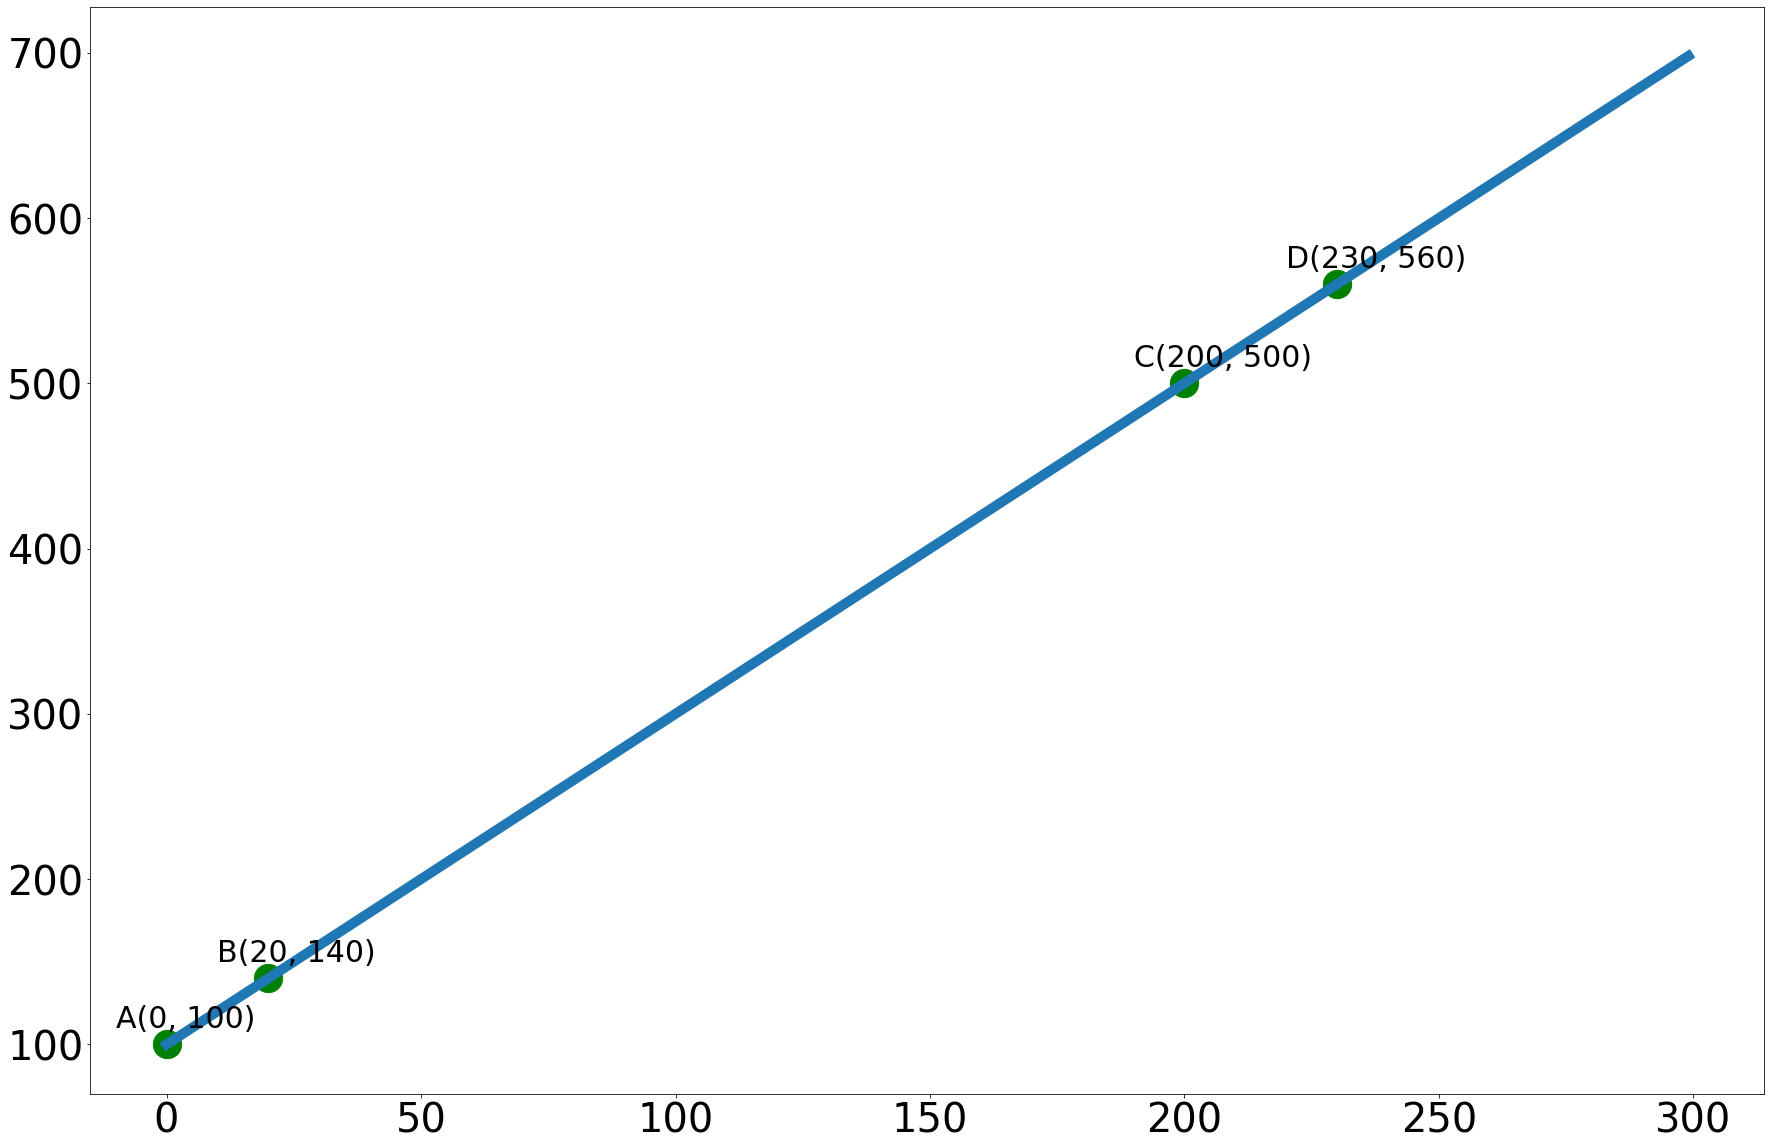
\includegraphics[scale=0.15]{chapter001/figures/fig003}
    \caption{The slope of A and B is the same as C and D}
    \label{fig:Fig3}
\end{figure}

\subsection{Example 1}
Given 2 lines which are represented by equations $f(x) = 5x + 3$ and $g(x) = 10x + 6$, respectively.

\begin{tabular}{ |p{3cm}||p{3cm}|p{3cm}|p{3cm}|}
 \hline
 \multicolumn{2}{|c|}{Investigating Steepness Values} \\
 \hline
 $f(x) = 5x + 3$ & $g(x) = 10x + 6$\\
 \hline
 $x=1, y=8$  & $x=1, y=16$\\
 $x=2, y=13$ & $x=2, y=26$\\
 $x=3, y=18$ & $x=3, y=36$\\
 $x=4, y=23$ & $x=4, y=46$ \\
 $x=5, y=28$ & $x=5, y=56$\\
 \hline
\end{tabular}
\\
The $g(x)$ is always rise faster than $f(x)$. The steepest lines are those for which the absolute value of the slope is the largest.

\section{Rates of Change}
\begin{figure}[h]
    \centering
    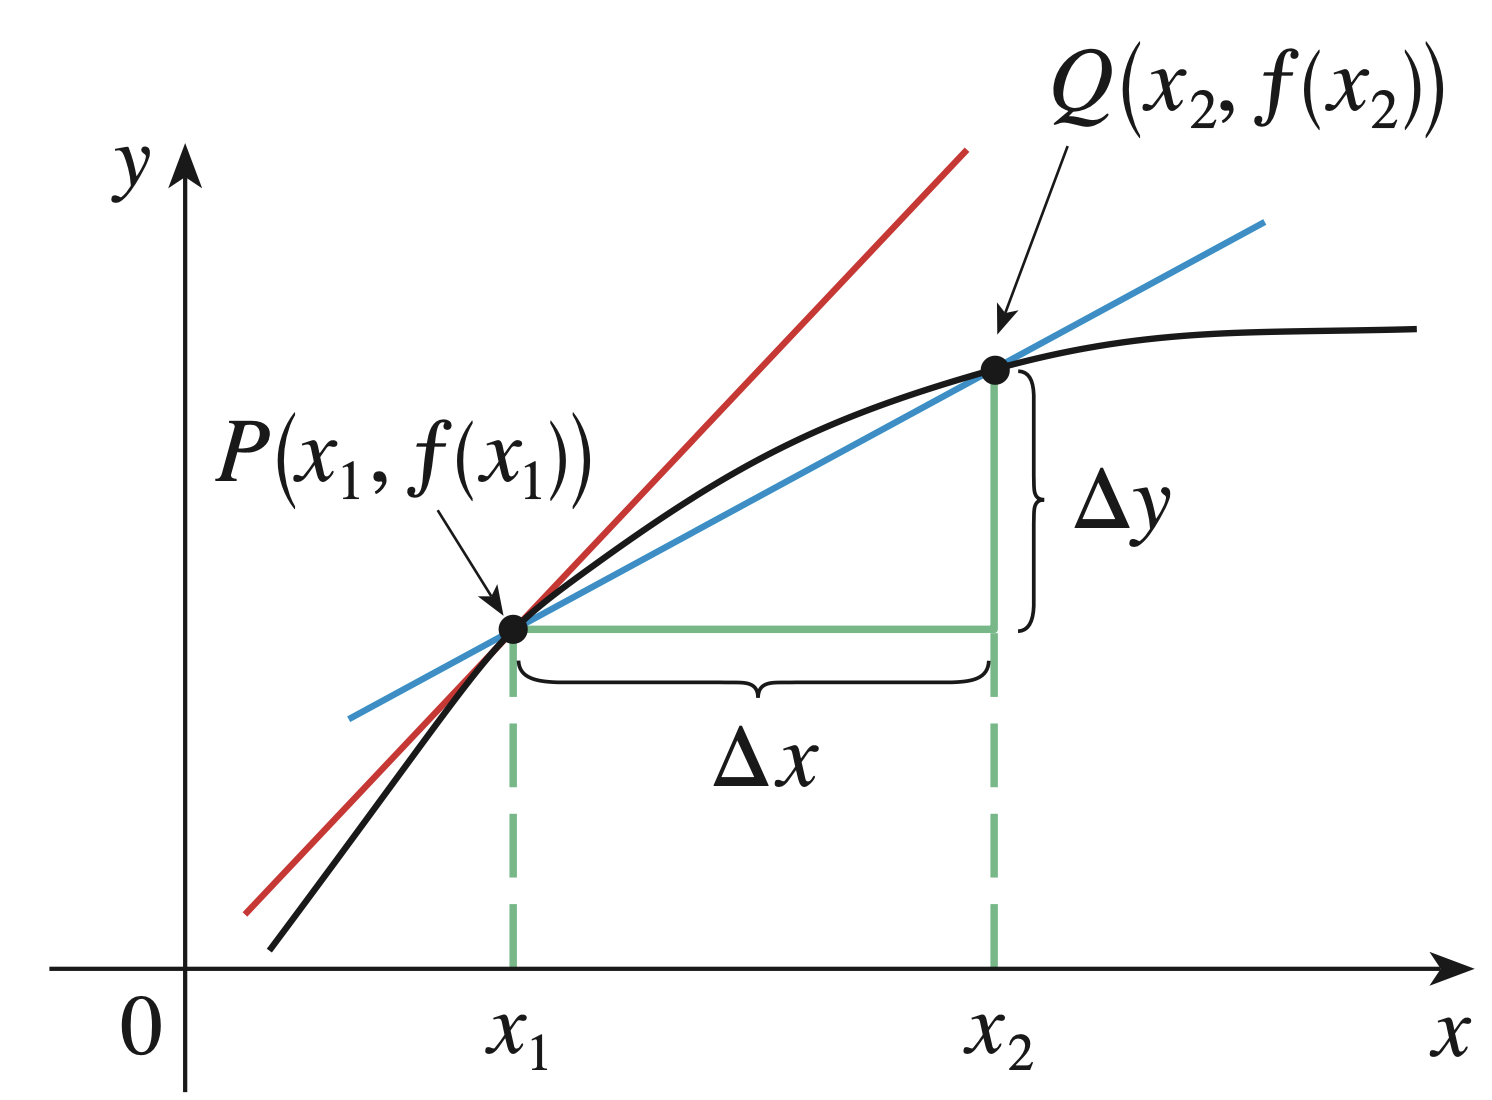
\includegraphics[scale=0.3]{chapter001/figures/fig004}
    \caption{Rates of Change}
    \label{fig:Fig4}
\end{figure}

\begin{flushleft}
Given a function $y=f(x)$, if $x$ changes from $x_1$ to $x_2$, then the change in $x$ is $\Delta x = x_2 - x_1$ and the corresponding change in $y$ is $\Delta y = f(x_2) - f(x_1)$.
\end{flushleft}

\begin{flushleft}
The difference quotient

\begin{equation}
\label{eq:2}
\frac{\Delta y}{\Delta x} = \frac{f(x_2) - f(x_1)}{x_2 - x_1}
\end{equation}

is called the \textbf{average rate of change of y with respect to x} over the interval $[x_1, x_2]$ and can be interpreted as the slope of the secant line $PQ$ in Figure \ref{fig:Fig4}

We now consider the average rate of change over smaller and smaller intervals by letting $x_2$ approach $x_1$ and therefore letting $\Delta x$ approach 0.

The limit of these average rates of change is called the (\textbf{instantaneous}) \textbf{rate of change of $y$ with respect to $x$} at $x = x_1$, which is interpreted as the slope of the tangent to the curve $y = f(x)$ at $P(x_1, f(x_1))$
\end{flushleft}

\begin{equation}
\label{eq:3}
instantaneous\ rate\ of\ change = \lim_{\Delta x \to 0} \frac{\Delta y}{\Delta x} = \lim_{x_2 \to x_1} \frac{f(x_2) - f(x_1)}{x_2 - x_1}
\end{equation}

\begin{flushleft}
We recognize this limit as being the derivative $f'(x_1)$.
we know the one interpretation of the derivative $f'(a)$ is as the slope of the tangent line to the curve $y=f(x)$ when $x=a$
\end{flushleft}

\begin{mybox}{Derivative}
The derivative $f'(a)$ is the instantaneous rate of change of $y=f(x)$ with respect to $x$ when $x = a$.
\end{mybox}

\begin{flushleft}
The connection with the first interpretation is that if we sketch the curve $y = f(x)$, then the instantaneous rate of change is the slope of the tangent to this curve at the point where $x = a$.

This means that when the derivative is large, the y-values change rapidly. When the derivative is small, the curve is relatively flat (as at point $Q$) and the y-values changes slowly.
\end{flushleft}

\subsection{Measuring the Rate of Increase of Blood Alcohol Concentration}
Biomedical scientists have studied the chemical and physiological changes in the body that result from alcohol consumption. The reaction in the human body occurs in two stages: a fairly rapid process of absorption and a more gradual one of metabolism. Biomedical scientists have studied the chemical and physiological changes in the body that result from alcohol consumption. The reaction in the human body occurs in two stages: a fairly rapid process of absorption and a more gradual one of metabolism.

Medical researchers measured the blood alcohol concentration (BAC) of eight fasting adult male subjects after rapid consumption of $15 mL$ of ethanol (corresponding to one alcoholic drink).1 The data they obtained were modeled by the concentration function. The graph of C is shown in Figure \ref{fig:Fig5}

\begin{equation}
\label{eq:4}
C(t) = 0.0225te^{-0.0467t}
\end{equation}

where $t$ is measured in minutes after consumption and $C$ is measured in $mg/mL$. How quickly is the BAC increasing after 10 minutes?

\begin{figure}[h]
    \centering
    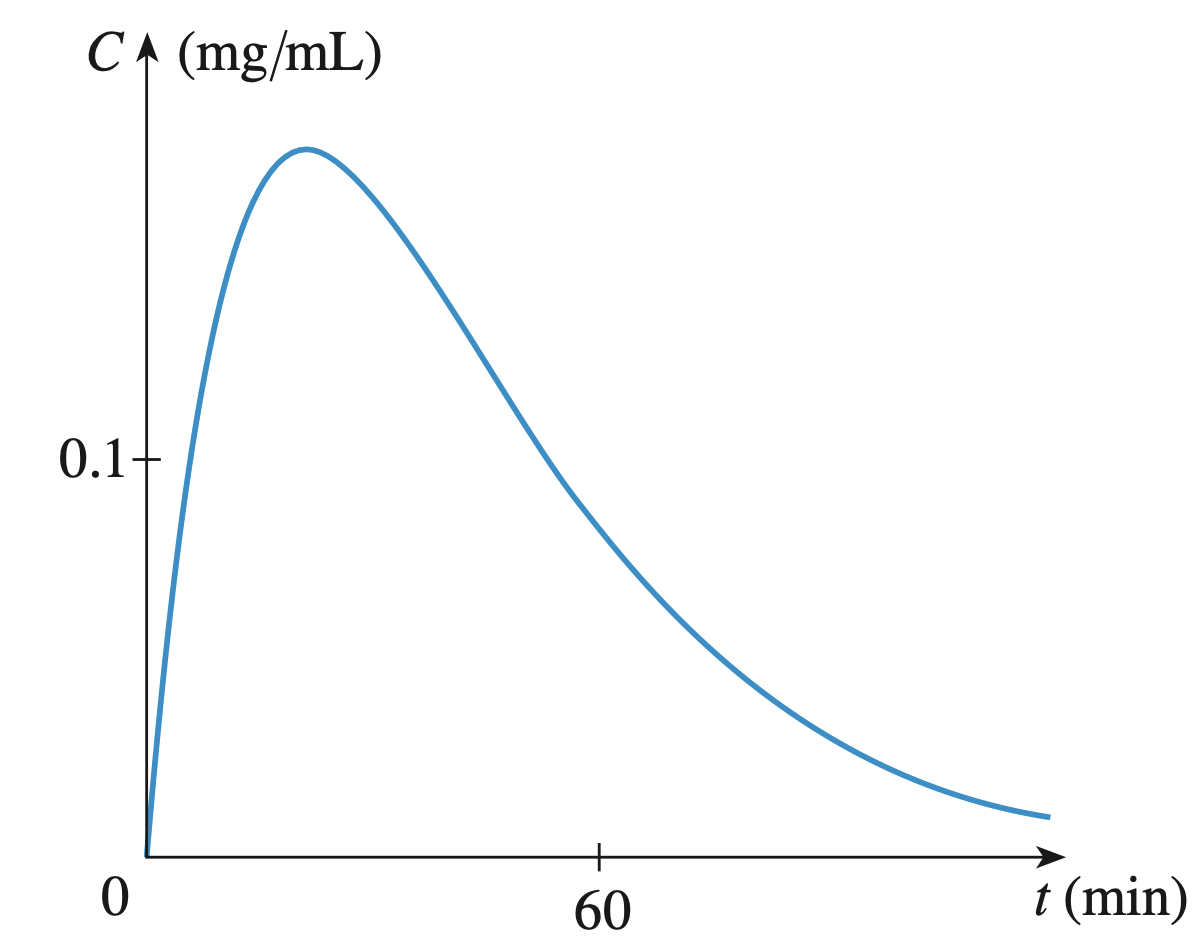
\includegraphics[scale=0.3]{chapter001/figures/fig005}
    \caption{Blood Alcohol Concentration}
    \label{fig:Fig5}
\end{figure}

\begin{tabular}{ |p{3cm}||p{3cm}|p{3cm}|p{3cm}|}
 \hline
 \multicolumn{2}{|c|}{Investigating Steepness Values} \\
 \hline
 Time interval & Average rate of change\\
 \hline
 $10 \leq t \leq 11$    & 0.00703\\
 $10 \leq t \leq 10.5$  & 0.00727\\
 $10 \leq t \leq 10.1$  & 0.00747\\
 $10 \leq t \leq 10.01$ & 0.00751 \\
 $9 \leq t \leq 10$     & 0.00804\\
 $9.5 \leq t \leq 10$   & 0.00777\\
 $9.9 \leq t \leq 10$   & 0.00757\\
 $9.99 \leq t \leq 10$  & 0.00752\\
 \hline
\end{tabular}

\begin{flushleft}
It appears that as we shorten the time period, the average rate of change is becoming closer and closer to a number between 0.00752 and 0.00753 (mg/mL)/min. The instantaneous rate of change at t = 10 is defined to be the limiting value of these average rates of change over shorter and shorter time periods that start or end at t = 10. So we estimate that the BAC increased at a rate of about 0.0075 (mg/mL)/min.

we estimated that the rate of increase of the blood alcohol concentration when $t = 10$ is about 0.0075 (mg/mL)/min. The equation of the curve is \ref{eq:4} which gives $C(10) \approx 0.14105$. So, using the point-slope equation of a line, we get that an approximate equation of the tangent line at $t=10$ is 
\end{flushleft}

\begin{equation}
\label{eq:5}
C - 0.14105 = 0.0075(t - 10)
\Leftrightarrow C = 0.06605 + 0.0075t
\end{equation}

\subsection{Malarial parasites}
The following table, supplied by Andrew Read, shows experimental data involving malarial parasites. The time t is measured in days and N is the number of parasites per micro-liter of blood.

\begin{tabular}{ |p{3cm}||p{3cm}|p{3cm}|p{3cm}|}
 \hline
 \multicolumn{2}{|c|}{Investigating Steepness Values} \\
 \hline
 t & N\\
 \hline
 1    & 228\\
 2    & 2,357\\
 3    & 12,750\\
 4    & 26,661\\
 5    & 372,331\\
 6    & 2,217,441\\
 \hline
\end{tabular}

\begin{flushleft}
(a) Find the average rates of change of N with respect to t over the intervals [1, 3], [2, 3], [3, 4], and [3, 5].\\
(b) Interpret and estimate the value of the derivative N'(3).
\end{flushleft}

\subsubsection{Solution}

\begin{flushleft}
(a) The average rate of change over [1, 3] is
$$\frac{N(3) - N(1)}{3 - 1} = \frac{12,750 - 228}{2} = 6261 (parasites/\mu L)/day$$
Similar calculations give the average rates of change in the following table:
\end{flushleft}


\begin{tabular}{ |p{3cm}||p{3cm}|p{3cm}|p{3cm}|}
 \hline
 \multicolumn{2}{|c|}{Investigating Steepness Values} \\
 \hline
 Interval & Rate of change\\
 \hline
 $[1, 3]$ & 6,261\\
 $[2, 3]$ & 10,393\\
 $[3, 4]$ & 13,911\\
 $[3, 5]$ & 179,791\\
 \hline
\end{tabular}

\begin{flushleft}
(b) The derivative $N'(3)$ means the rate of change of N with respect to $t$ when $t=3$ days.
	$$
		N'(3) = \lim_{\Delta t \to 3} \frac{N(t) - N(3)}{t - 3}
	$$
\end{flushleft}

\subsection{\href{https://www.slideshare.net/ichazalia/derivative-application-in-medical-and-biology}{Growth Rate of Tumor}}

\begin{flushleft}
This example is recommended by \cite{azalia}.\\
There are 3 certain levels of a tumor regarding to its malignancy.
\begin{enumerate}
    \item The first level is benign tumor. It does not invade nearby or spread to other parts of the body.
    \item The second level is premalignant or precancerous tumor which is not yet malignant, but is about to become so.
    \item The last level is malignant tumors. These are cancerous tumors, they tend to become progressively worse, and can potentially result in death.
\end{enumerate}

The rate at which a tumor grows is directly proportional to its volume. Larger tumors grow faster and smaller tumors grow slower.
The volume of a tumor is found by using the exponential growth model which is
	$$
		V(t) = V_0 \cdot e^{kt}
	$$
	where
	
\begin{enumerate}
    \item $V_0$ = initial volume.
    \item e     = exponential growth (2.7182...)
    \item k     = growth constant
    \item t     = time
\end{enumerate}

(a) Find the rate of change of a tumor when its initial volume is $10cm^3$ with a growth constant of 0.075 over a time period of 7 years.\\
(b) Find the rate of change of a tumor when its initial volume is $2cm^3$ with a growth constant of 0.075 over a time period of 7 years.
\end{flushleft}

